\documentclass{article}%
\usepackage[T1]{fontenc}%
\usepackage[utf8]{inputenc}%
\usepackage{lmodern}%
\usepackage{textcomp}%
\usepackage{lastpage}%
\usepackage[head=40pt,margin=0.5in,bottom=0.6in]{geometry}%
\usepackage{graphicx}%
%
\title{\textbf{¿Con qué cuenta Juan Guaidó en su regreso a Venezuela?}}%
\author{EL NACIONAL}%
\date{04/03/2019}%
%
\begin{document}%
\normalsize%
\maketitle%
\textbf{URL: }%
http://www.el{-}nacional.com/noticias/politica/con{-}que{-}cuenta{-}juan{-}guaido{-}regreso{-}venezuela\_273305\newline%
%
\textbf{Periodico: }%
EN, %
ID: %
273305, %
Seccion: %
Política\newline%
%
\textbf{Palabras Claves: }%
NO\_TIENE\newline%
%
\textbf{Derecho: }%
2.1%
, Otros Derechos: %
\newline%
%
\textbf{\textit{La Unión Europea, que ha demostrado su precupación ante la situación del país, advirtió a Nicolás Maduro tomar una "firme condena" en su contra si arresta a Guaidó}}%
\newline%
\newline%
%
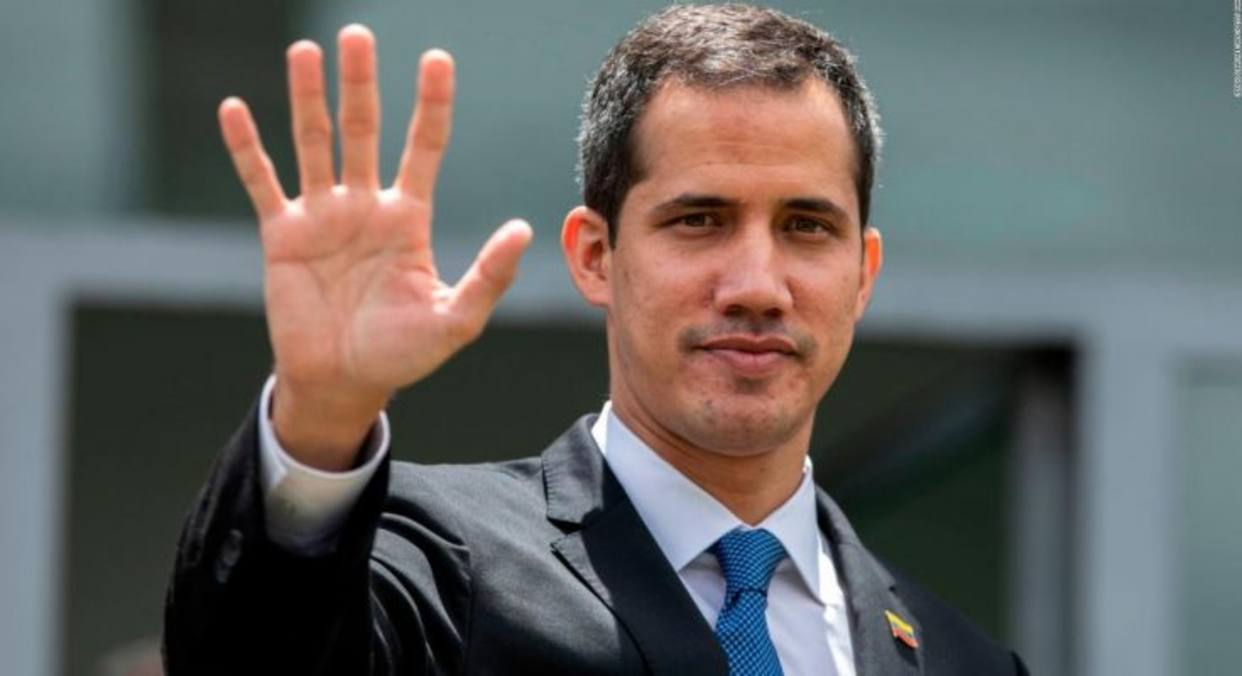
\includegraphics[width=300px]{EN_273305.jpg}%
\newline%
%
Juan Guaidó, presidente interino de Venezuela, informó que este lunes estaría de regreso a su país.Para lograr su retorno el político cuenta con el apoyo de los gobiernos latinoamericanos y con una tajante advertencia de Europa en la que ofrecen una condena internacional “firme” a Nicolás Maduro si toma medidas de arresto en su contra.%
\newline%
%
Es una incógnita pensar cómo ingresará Guaidó a Venezuela: ¿los militares impedirán su paso?, ¿lo encarcelarán?, ¿o ya se encuentra en el país? No han anunciado su llegada, pero lo que sí se sabe son las cinco armas con las que cuenta el mandatario interino para lograr un regreso exitoso.%
\newline%
%
A continuación, la lista presentada por el portal~Al Navío:%
\newline%
%
1. Cuenta con el apoyo de los mandatarios de Latinoamérica desde que el 23 de enero realizó la juramentación en una multitudinaria marcha en la ciudad de Caracas.%
\newline%
%
2. Tiene una oposición unida tras consolidarse como líder de la Asamblea Nacional también en el mes de enero.%
\newline%
%
3. El papel de la Asamblea Nacional, quienes le concedieron el permiso de salir del país y luego lo prorrogaron.%
\newline%
%
4. Cuenta con los venezolanos, de quienes se espera una movilización masiva este lunes para recibirlo y respaldarlo con su apoyo.%
\newline%
%
5. Europa, una región que ha advertido a Nicolás Maduro tomar una “firme condena” si se toman medidas carcelarias contra Guaidó.%
\newline%
%
Lea más~aquí.%
\newline%
%
\end{document}